% Paul Meyer-Rachner, paul@meyer-rachner.email 

%%%%%%%%%%%%%%%%%%%%%% DOCUMENT PARAMETERS %%%%%%%%%%%%%%%%%%%%%%%

\documentclass[usletter, 11pt]{extarticle}
\usepackage{report_mystyle}
\usepackage{parskip}
\usepackage{tabularx}
\usepackage{mdframed}
\usepackage{calligra}

\title{Neurodetect: On-chip Biosignal Computation for Health Monitoring}

\newcommand{\seprule}[0]{\vspace{9pt} \hrule}

\setlength{\columnseprule}{0.2pt} 

%%%%%%%%%%%%%%%%%%%%%% BEGIN DOCUMENT %%%%%%%%%%%%%%%%%%%%%%%%%%%%
\linespread{1.1}

\begin{document}

%%%%%%%%%%%%%%%%%%%%%% CUSTOMIZATION %%%%%%%%%%%%%%%%%%%%%%%%%%%%%

% space between bottom of text and footer
\setlength{\footskip}{20pt}

% Title
\maketitle

\begin{center}
{\large Capstone Project Final Report}\\[0.5cm]
    \text{Chen Fu, Sherwin Lau, Mary Lee Lawrence, Paul Meyer-Rachner, Jingbo Wu}
    \text{Advisor: Professor Rikky Muller}\\[0.5cm]
    \text{University of California, Berkeley} \\
    \text{Department of Electrical Engineering and Computer Science} \\
    \text{May 2018}\\[0.5cm]
\end{center}

\vspace{11pt}% add some vertical space

%%%%%%%%%%%%%%%%%%%%%% BEGIN TEXT %%%%%%%%%%%%%%%%%%%%%%%%%%%%%%%%

\emph{}

\begin{mdframed}
\textsc{Executive Summary}

Epilepsy is a serious neurological disorder affecting around 1\% of the world’s population. Patients experience recurring seizures that greatly degrade their quality of life. While current therapies such as anti-epileptic drugs and resective surgery have done a great deal to make life manageable for patients by reducing the number of seizures experienced, they are not always effective. Emerging treatment with neurostimulation and localized drug delivery has been shown to be efficacious in stopping seizures in the brain before patients present symptoms. However, these methods rely on accurate seizure detection to provide in-the-moment treatment. Neurodetect created a seizure detection algorithm that, when combined with stimulation or drug delivery, will be a closed-loop system to treat patients with epilepsy. Our detection algorithm uses a matrix of multiple features from intracranial encephalogram (iEEG) data, including line length and power spectral density, to improve the detection of seizures when compared to using single features. Previous research into aggregation of multiple features has demonstrated the efficacy of this method \cite{donos2015}. Preliminary results show that by assigning different weights to different features, we are able to tune the algorithm to provide the best detection on a patient-by-patient basis. 
\end{mdframed}
		
\newpage
\vspace{11pt}
\textsc{Introduction}
\vspace{11pt}

Neurodetect is an implantable microchip that monitors the brain’s electrical activity through iEEG to detect seizures. This kind of device is used in a closed-loop system to trigger neurostimulation or drug release within the brain to treat a seizure, thereby enabling epileptic patients that are not responsive to common therapies (antiepileptic drugs or resective surgery) to lead more normal lives. Our capstone’s goal is to design the seizure detection algorithm and to implement it in hardware. \\

This paper first explains the motivations behind our project before moving to exploring the current state-of-the-art in seizure detection and analyzing the success of the different algorithms in terms of their detection metrics and hardware specifications. By further looking at the features used to analyze the iEEG data, we develop a foundation of comparison to our device. This paper next focuses on the technical aspects of the project and provides background on our current research in both software and hardware.

\vspace{11pt}
\textsc{Section 1 – Engineering Leadership}
\vspace{11pt}

\textbf{Epilepsy is a common disease that greatly decreases the quality of life} 

About 1 in 26 people will develop epilepsy in their lifetime \cite{mayoclinic}, making it the second most common neurological disorder \cite{donos2015}. Epilepsy patients experience recurrent seizures, events where a large group of neurons in the brain fires off wrong signals \cite{mediline}. Patients manifest various symptoms ranging from temporary confusion and staring spells to uncontrollable jerking movements or even loss of consciousness.

The unpredictable nature of seizures, combined with their deleterious symptoms, has a huge impact on the daily life of epilepsy patients. People diagnosed with epilepsy often are prohibited from driving. Other activities like swimming or riding a bike can quickly become dangerous if a patient experiences a seizure. Studies have shown that epilepsy increases the risk of accidents by approximately 50\%  \cite{beghi2002} and 15\% of all deaths in epilepsy patients are related to seizures \cite{shorvon1996}. Furthermore, people with epilepsy are more likely to suffer from depression and anxiety, and to commit suicide \cite{kerr2012}.

On average, the time to remission for epilepsy patients is 10 years \cite{shorvon1996}. Luckily, there are currently several different therapies for epilepsy that potentially improve the quality of life for patients.

\vspace{11pt}
\textbf{Existing therapies can be effective but do not work for everyone}

While there is no cure for epilepsy, existing therapies can help patients manage their symptoms. Current therapies include antiepileptic drugs (AEDs), neurostimulation and resective surgery (as presented in Table 1).

AEDs fully prevent seizures in about 33\% of patients and decrease the frequency of seizures in another 20\% of patients \cite{shorvon1996}. However, since only a fraction of the administered drug passes the blood-brain barrier, high drug doses are required, leading to serious side effects like nausea, sleepiness and decrease in cognitive capabilities. Therefore, while AEDs provide a way to prevent seizures or reduce their number, the side effects associated with them make them an unpopular choice \cite{kerr2012}.

Another possible therapy is neurostimulation. This approach consists of electrically stimulating the area of the brain where seizures occur. Over a longer treatment period, neurostimulation can reduce the number of seizures by 50\% to 69\% \cite{muller2016}. However, the drawback of this treatment is that over time the neurons can become desensitized to stimulation, ultimately lowering efficacy \cite{logesparan2012}. Furthermore, this approach does not work for all patients.

Finally, some patients with very localized seizures are candidates for resective surgery, which consists in removing the part of the brain responsible for the seizures. However, this is a small minority of patients and not effective for the general population suffering from epilepsy.

The drawbacks of current therapies demonstrate that there is room for expansion and further research into the efficacy of implantable devices to treat epilepsy.

\begin{table}[!h]
	\centering
	\begin{tabularx}{\textwidth}{X|X|X}
		& \textbf{Advantage} & \textbf{Disadvantage} \\ \hline \hline
		\textbf{Anti-epileptic Drugs} & Can fully prevent seizures & High dosage to pass blood-brain barrier leads to serious side effects, effectiveness varies from patient to patient \\ \hline
		\textbf{Resective Surgery} & Perpetually prevents seizures in patients with very localized seizures & Small minority of patients \\ \hline
		\textbf{Neurostimulation} & Very effective in reducing the number of seizures & Over time neurons can be desensitized, reducing efficacy \\ \hline
		\textbf{Implantable Detection Device (this paper)} & Effective at detecting and mitigating seizures & Invasive
	\end{tabularx}
	\caption{Comparison of different treatment options.}
\end{table}

\vspace{11pt}
\textbf{Implantable detection devices can be used to stymie seizures}

A relatively new therapy being researched for epilepsy treatment uses implantable microchips to detect the patient’s seizures. These chips are placed under the skull on the surface of the brain and, through several electrodes placed within the skull, measure iEEG, the electrical activity between neurons. iEEG provides high quality measurements that are less prone to outside disturbances than other recording methods. Seizures are characterized by a spike in neural activity, which the chip can detect. It can then initiate the release of drugs directly within the brain or trigger neurostimulations, both of which result in cessation of the seizure. One obvious benefit to this approach is since the implantable device is within the blood brain barrier, the drugs can be released in lower doses thus avoiding side effects. The relatively low maintenance costs of these devices also means that epilepsy has less of an impact on the day-to-day lives of patients. 

As of 2015, there was only one approved device for direct electrical brain stimulation for epilepsy \cite{thomas2015}. NeuroPace is a small, implantable responsive neurostimulator system that consists of a processor, battery and two small leads, with an area of 4 x 6 x 0.7cm (Wu, 2018). The battery in the system lasts an average of 3 years before it has to be replaced \cite{neuropace}. The system first detects the onset of seizures via the iEEG signals. Once it detects that the patient is having a seizure, it reacts by electrically stimulating the focus of the seizure to treat the seizure. The system is able to learn the seizure patterns for each patient over time, and further improve its detection algorithm. By year 3 of use, it can reduce up to 60\% of seizures, and up to 72\% by year 7. The system has been evaluated in 3 clinical trials totaling 1700 years of patient experience with the device \cite{neuropacetrial}.

\vspace{11pt}
\textbf{The selection of iEEG features is critical for detecting seizures}

Both EEG and iEEG based sensing systems can be implemented for seizure detection 
\cite{altaf2015, shoaran2016}. While EEG has the advantage of being non-invasive, drawbacks include low resolution and high sensitivity to noise from the surrounding environment.

iEEG based detection systems, like Neurodetect, can ensure higher detection accuracy, but implantable devices are constrained by a tight energy and space budget. The computational complexity of the detection algorithm directly impacts the power consumption, so a more complex algorithm puts more strain on the energy budget. After evaluating the performance and computational complexity of different features, we decided to use features such as line length, spectral band power and nonlinear energy to determine if a seizure occurred.

While there are many other features that can be calculated, such as autocorrelation and amplitude (see Table \ref{tab:overview}), line length and spectral band power are features best suited for seizure detection on a microchip since they reliably detect seizures while having a relatively low computational complexity \cite{logesparan2012}. Once different features are calculated from the iEEG data, they are benchmarked against a preset threshold to determine if there is a seizure. Typically, more than one feature is used in order to improve the accuracy of the system.

\begin{table}[h!]
	\centering
  	\begin{tabularx}{\textwidth}{|X|X|X|X|X|X|X|}
  		\hline
	    & \cite{altaf2015} & \cite{oleary2018} & \cite{shoaran2016} & \cite{donos2015} & \cite{raghunathan2009} & \textbf{This work} \\ \hline
	    Technology (nm) & 180 & 130 & 180 & - & 180 & 32 \\ \hline
	    Data & EGG & iEEG & iEEG & iEEG & iEEG & iEEG \\ \hline
	    Channels & 16 & 32 & 16 & 1 & 1 & 16 \\ \hline
	    Features & Linear support-vector machine  classifiers & Signal-band energy, phase locking value, cross frequency coupling & Signal power, line length, Autocorrelation, MAV(ABS) & Eleven features in time and frequency domain & Time and frequency information combined with amplitude of recorded LFP data & Line length, nonlinear energy, power spectrum density \\ \hline
	    Power & 2.73 $\mu$J/class & 674.4 $\mu$W & 0.92 $\mu$W/ch & - & <350 nW & 32 nW\\ \hline
	    Area & 25mm$^2$ & - & 1.1mm$^2$ & - & - & - \\ \hline
	    Sensitivity & 95.7\% & 100\% & 100 \% & 86.27\% & 95.3 \% & 86 \% \\ \hline
	    False Alarm Rate & 0.27/hr & 0.81/hr & 0.15/hr & 0.33/hr & - & 0.83/hr\\ \hline
	    Detection Delay & 1s & - & 0.5s & 5.47s & 8.5s & 8.75s \\ \hline
  	\end{tabularx}
  	\caption{Overview of the results of different papers on real-time seizure detection.}
  	\label{tab:overview}
\end{table}

\vspace{11pt}
\textbf{Designing a device that is implantable comes with additional constraints}

Key hardware metrics of success in the design of seizure detection system-on-a-chip (SoC) include the size and power consumption. The size of the SoC is constrained; the chip must be small since it is an implantable device. Typical state-of-the-art designs range from 1mm2 to 25mm2 \cite{shoaran2016}. It also must be low power to reduce the need to replace the battery or constantly charge the device.

There are also many design constraints within the algorithm itself, including sensitivity, the false alarm rate (FAR) and detection latency. Sensitivity and FAR are the key metrics that we considered most important when designing our seizure detection algorithm. The sensitivity of a system indicates the percentage of seizures that are correctly detected. Several designs have achieved sensitivities of over 95\%. However, this sensitivity can come at the cost of greater number of false alarms. The FAR indicates how many times in an hour the algorithm identifies something as a seizure when it is not. A comparable measure is the specificity which indicates the percentage of normal activity that is correctly identified and not falsely identified as a seizure. Different designs may lead to very different FAR values due to differences in the algorithm as well as in the testing environments \cite{shoaran2016}.

Another important constraint is detection (or system) latency, i.e. how long the system takes to respond once it has detected a seizure. Most implantable seizure detection systems are closed loop systems combined with drug delivery or neurostimulation, thus shorter latency means that the seizure is treated more quickly and the patient is less likely to exhibit symptoms.

While Table \ref{tab:overview} presents an overview of typical reported performance for seizure detection, most papers do not offer a lot of background on how these numbers are calculated. This means that there are limitations in our ability to compare results across devices and with our own device. 

\vspace{11pt}
\textbf{Finding high quality iEEG data can be challenging since most of them are proprietary}

iEEG data from epileptic patients is essential in testing Neurodetect's algorithms. However, obtaining iEEG data can be challenging since the process involves performing brain surgery to place electrodes and recording device on the brains of willing participants. This is often a lengthy and costly process, thus most entities that went through it are not willing to freely share their data.

The data we used is hosted on the iEGG.org \cite{ieegorg} website.
IEEG.org is an initiative funded by the National Institute of Neurological Disorders and Stroke. The data includes iEEG measurements across several channels and the seizures have been annotated within the data by a physician. This allows to evaluate the effectiveness of Neurodetect's algorithms at recognizing correct seizures. However, the quality of the data varies. There is a lot of data is available for free on IEEG.org, but it can be challenging to pick correctly annotated and accurate data since this data is user-contributed.

\vspace{11pt}
\textsc{Section 2 – Technical Contributions}
\vspace{11pt}

\begin{figure}[!h]
	\centering
	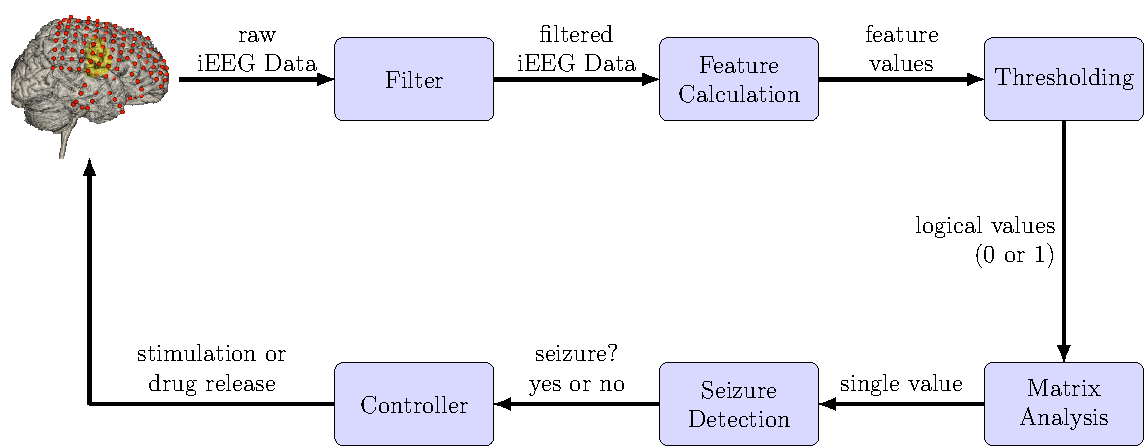
\includegraphics[width = \textwidth]{img/overview_diagram.pdf}
	\caption{General overview of Neurodetect's components.}
	\label{fig:overview_diagram}
\end{figure}
 
The Neurodetect chip is composed of multiple computation modules, each of which represents one of the processing steps applied to the iEEG data. Figure \ref{fig:overview_diagram} illustrates this. The data acquired by the sensors is filtered, featurized, compared to a threshold and then stored in a matrix. This matrix is then used to detect a seizure. All these steps were first designed in software before being implemented in hardware.

\vspace{11pt}
\textsc{Section 2.1 – Software Seizure Detection Algorithm}
\vspace{11pt}

The raw iEEG data acquired by the sensors goes through five processing steps. These steps are listed in figure \ref{fig:software_diagram} and are detailed hereafter. All steps are implemented using the computational software MATLAB.

\begin{figure}[p]
	\centering
	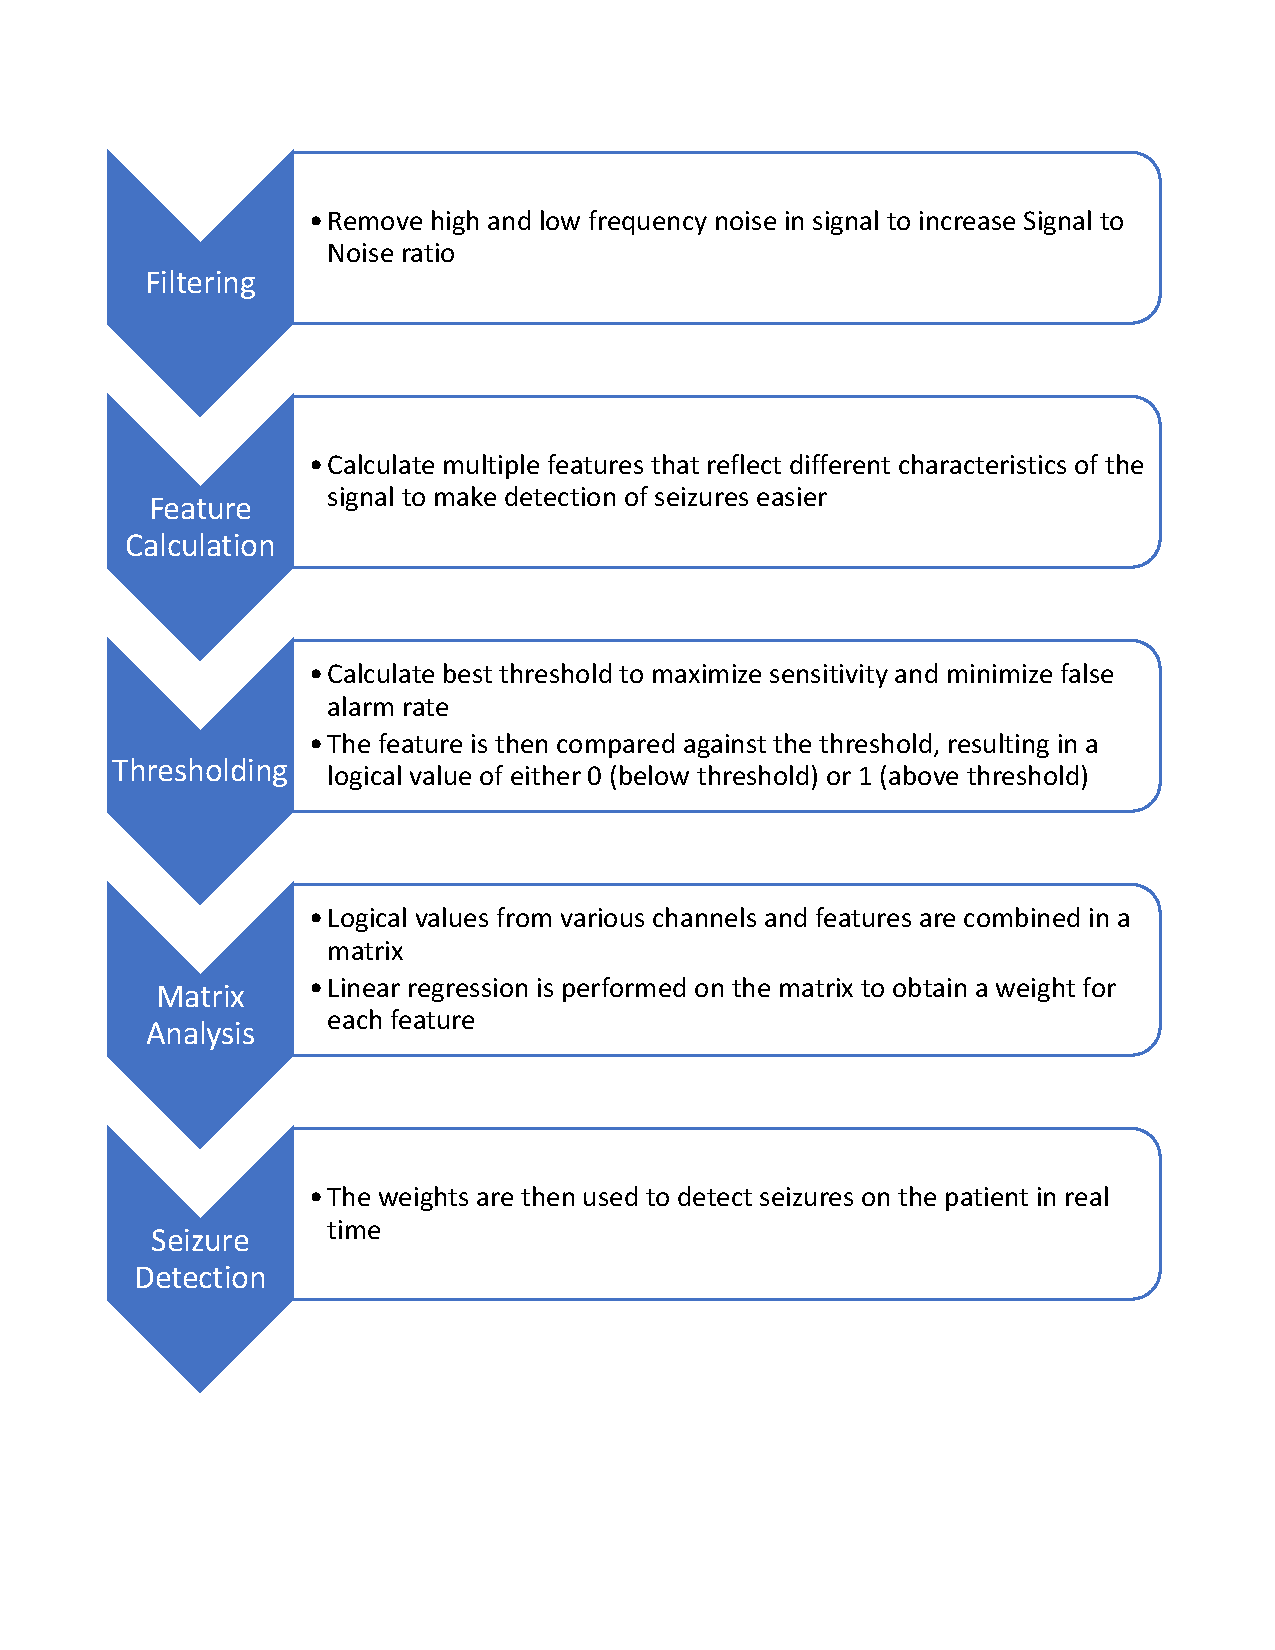
\includegraphics[width = \textwidth]{img/Round6_SoftwareDiagram}
	\caption{Overview of the software flow the iEEG signal is going through.}
	\label{fig:software_diagram}
\end{figure}

\vspace{11pt}
\textbf{Noise can lead to false alarms}

To remove noise in the low and high frequencies, the iEEG signal is first filtered using a 1 to 70 Hz bandpass filter. This increases the signal to noise ratio by removing the impact of internal and external noise sources like cardiac signals or electromagnetic waves emitted by electronic devices \cite{repovs2010}. This step is important because noise in the measurement can result in our algorithm wrongly detection a seizure. 

\vspace{11pt}
\textbf{Different features reflect different characteristics of the iEEG signal}

After filtering, several features are extracted from the iEEG signal. Features can be thought of as different attributes of the data, i.e. amplitude, variance can be 2 different features of the same data.  Initially, 10 features that were most used in literature were tested on 388.5 hours of iEEG recordings containing 108 seizures. To reduce computational complexity, the top 6 features that performed best were then selected to be part of the seizure detection algorithm. These features are
\begin{itemize}
	\item Line Length - a measure of how quickly the signal changes over time, both in amplitude and frequency
	\item Nonlinear Energy - a measure of the signal’s energy that is proportional to the non-linear component in the signal
	\item Power in the full spectrum - the energy of the signal over all frequencies 
	\item Power in three frequency bands - a measure of the amount of energy the signal has in specific frequency bands. The top performing frequency bands chosen were theta band (4-8 Hz), alpha band (8-14 Hz) and beta band (14-32 Hz).
\end{itemize}
All features are calculated over a one second long sliding window that is updated every 0.1s. This means that the above features are calculated once every 0.1s, using data that was obtained from the sensors over the last second.

\vspace{11pt}
\textbf{Every feature is compared against a threshold to detect seizures}

Next, each feature is compared against a threshold, in which if the feature value exceeds the threshold, a seizure is said to have occurred. To determine the best threshold, the number of detected seizures and false alarms were calculated for different threshold values, and the threshold that results in the highest detection accuracy and the lowest false alarm rate is taken to be the best threshold.

Once the best threshold is determined, the feature is compared against it and converted to logical values, i.e. 0 when feature value is below the threshold and 1 when above. This is done for every feature and every channel measured. One channel corresponds to one electrode inside the brain and therefore using multiple channels enables the analysis of iEEG signals across different locations of the brain. 

\vspace{11pt}
\textbf{Machine Learning can be used to improve detection accuracy}

After converting the features to logical values, the logical values of all features across all channels are then stored in a feature matrix. Each column of the matrix corresponds to a single feature and channel while each row corresponds to one sample. A sample is a measurement made at one point in time. The intuition behind analyzing multiple channels and features at once is that the occurrence of a seizure will likely be visible across multiple channels and features simultaneously, while noise that might lead to a false detection will in most cases be isolated to a few channels and features. Therefore, analyzing multiple channels and features can result in a higher sensitivity and lower FAR compared to only analyzing a single channel and feature.

In the next step, each feature is attributed a weight, which can be thought of as how good that specific feature is at detecting seizures. If a feature has a high weight, it means that this feature is good at detecting seizures. To detect seizures in real-time, a weighted sum is calculated by adding the logical value of every feature multiplied by its weight.

\begin{mdframed}
\begin{align*}
	\text{Weighted sum} &= \text{value of ch. 1  line length} \times \text{weight of ch. 1 line length} \\
	&+ \text{ value of ch. 1  alpha band power} \times \text{weight of ch. 1 alpha band power} \\
	&+ ...  \\
	&+ \text{ value of ch. 2  alpha band power} \times \text{weight of ch. 2 alpha band power} \\
	&+ ...  \\
\end{align*}
\end{mdframed}
If that weighted sum exceeds a certain threshold, a seizure is detected. This threshold can be changed depending on the desired sensitivity of the algorithm. A lower threshold results in the detection of more seizures but at the same time increases the false alarm rate. Inversely, a higher threshold yields less false alarms but lower sensitivity.

The weights are calculated using linear regression, more specifficaly the least squares procedure. Least squares is a machine learning algorithm that finds a best-fit linear model for the data. Weights obtained from the model are the optimal weights used to determine if a seizure has occurred or not.


\vspace{11pt}
\textbf{Using a weighted sum of features for seizure detections yield improved results
}

Results obtained from tests using machine learning on weighted features have shown that it achieves up to 60\% better results compared to just using a single feature and channel. Figure \ref{fig:sensitivity_plot_OLS} shows the tradeoff between achieved sensitivity and false alarm rate mentioned earlier. Different points on the curve are achieved by varying the detection threshold.

\begin{figure}[!h]
	\centering
	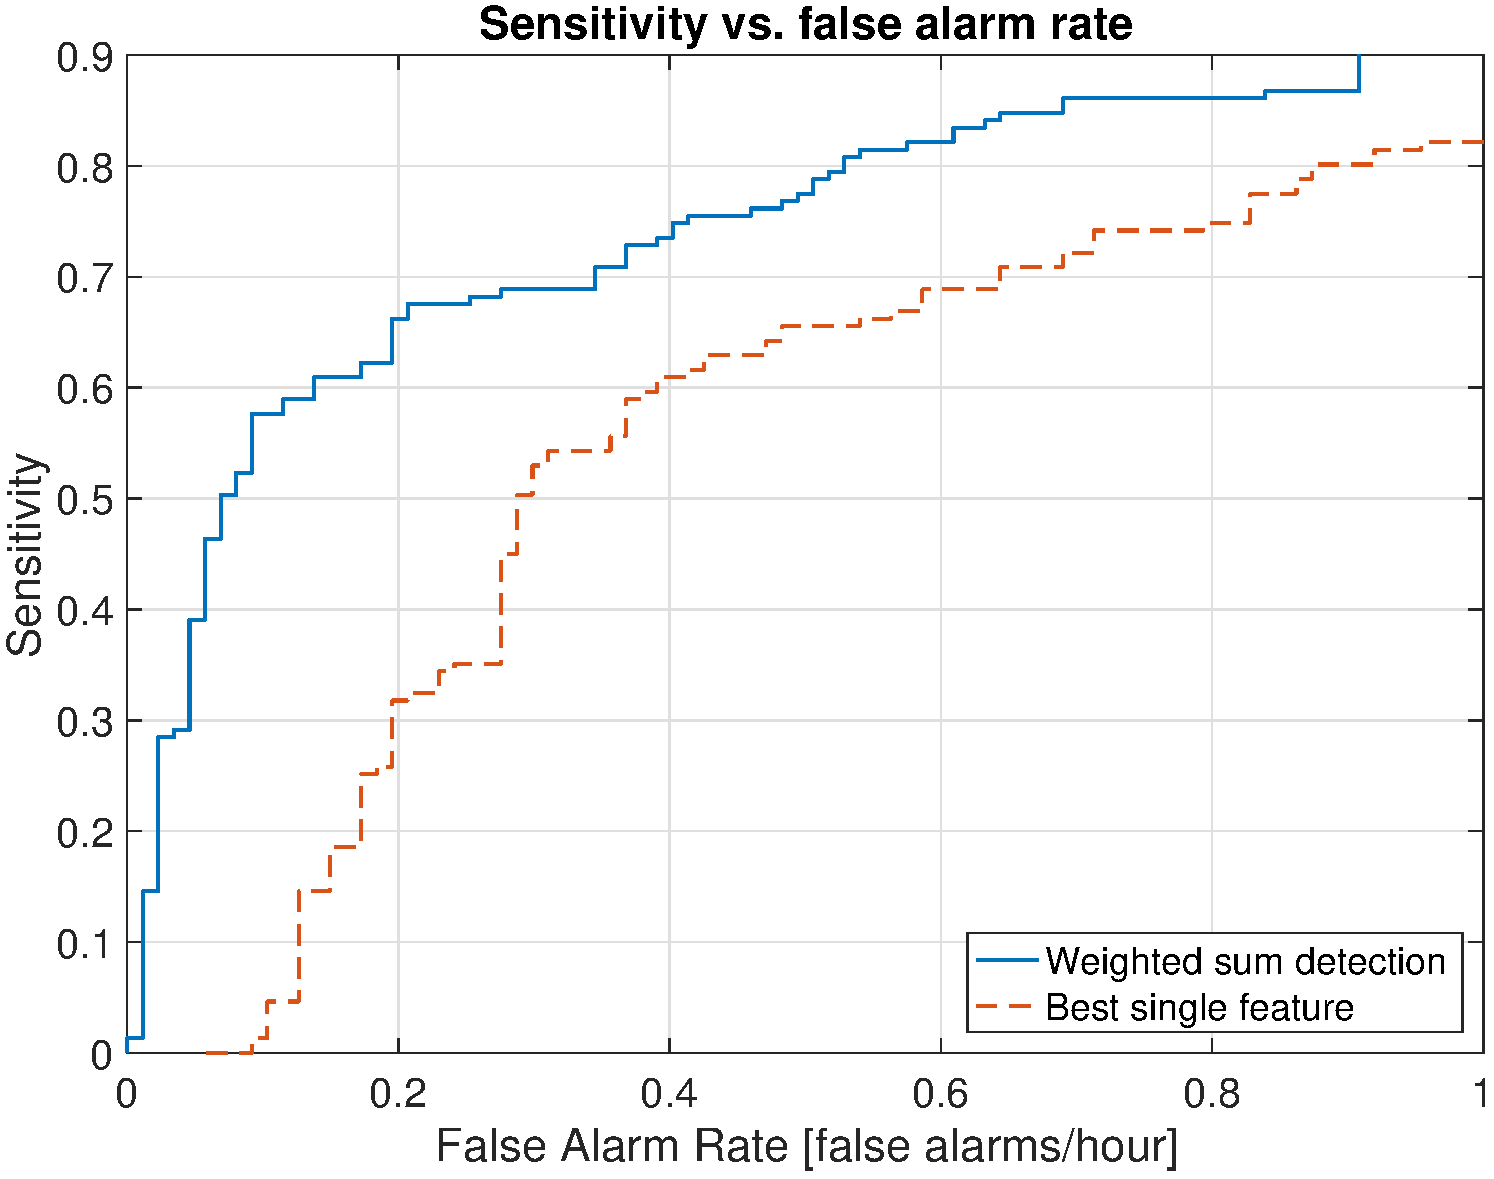
\includegraphics[width = 0.9\textwidth]{img/sensitivity_plot}
	\caption{Sensitivity vs. false alarm rate comparison plot. Each curve shows the maximum sensitivity achievable for a certain rate of false alarms, or conversely the minimum false alarm rate that has to be incurred to achieve a certain sensitivity. The solid blue line corresponds to the results when using the weighted sum while the orange dashed line corresponds the the results if only the single best feature is used.}
	\label{fig:sensitivity_plot_OLS}
\end{figure}

As can be seen in the plot, the curve obtained by using weighted sum is above the curve obtained by the single best feature. In other words, for a given sensitivity the weighted sum algorithm we will incur less false alarms.
 
In this patient’s case, for example, to achieve a sensitivity of 0.8 will mean that the FAR is 0.85 for a single feature, and only have 0.5 for the weighted sum. This means that the weighted sum incurs 60\% less false alarms per hour.

\vspace{11pt}
\textbf{A feature matrix allows the algorithm to be tailored for individual patients}

Another advantage of using the feature matrix combined with machine learning is that the weights given to each feature can be determined individually for every patient. Since seizure patterns vary widely across individuals, the algorithm used to detect seizures must also be optimized to suit the individual.

By calculating multiple features and then using least squares to determine the best weights for each feature, Neurodetect's seizure detection algorithm is tailored to suit to every individual patient. To do this, the optimal weights are calculated using the patient’s preliminary iEEG recordings. Such weights will vary from person to person, allowing Neurodetect's algorithm to adapt to the differences in seizure patterns.

\vspace{11pt}
\vspace{11pt}
\textbf{Not all features and channels contain useful information to detect seizures}

One interesting result from performing linear regression on the feature matrix is that majority of the optimal weights are 0 or close to 0. This effectively means that features and channels that get assigned a weight of 0 do not contain information relevant to detecting seizures as they do not play a part in the weighted sum. Therefore, such features and channels can be disabled on the chip, further reducing unnecessary computation and saving power. Indeed, Neurodetect's analysis has shown that using only the best 16 out of 96 features and channels results detection accuracy that is only 4\% worse than if all 96 were used. This means that the power consumption of the chip can be potentially reduced by over 80\%, thereby prolonging the battery life dramatically without significantly reducing the detection accuracy.

\clearpage
\textsc{Section 2.2 – Hardware Implementation}
\vspace{11pt}

After testing Neurodetect's seizure detection algorithm in software, the algorithm was implemented in hardware. The hardware prototype is created using a field-programmable gate array (FPGA). An FPGA is an integrated circuit which can be re-programmed, without the need to physically reroute actual wires, allowing for quick and flexible prototyping. The language used to program the FPGA is Verilog, which is an industry standard hardware description language (HDL). Verilog allows the designer to work in different abstraction levels such as at the register-transfer level (RTL), which is used for Neurodetect's design. Figure \ref{fig:hardware_diagram} illustrates the overall idea of the general hardware design and test flow.

\begin{figure}[!h]
	\centering
	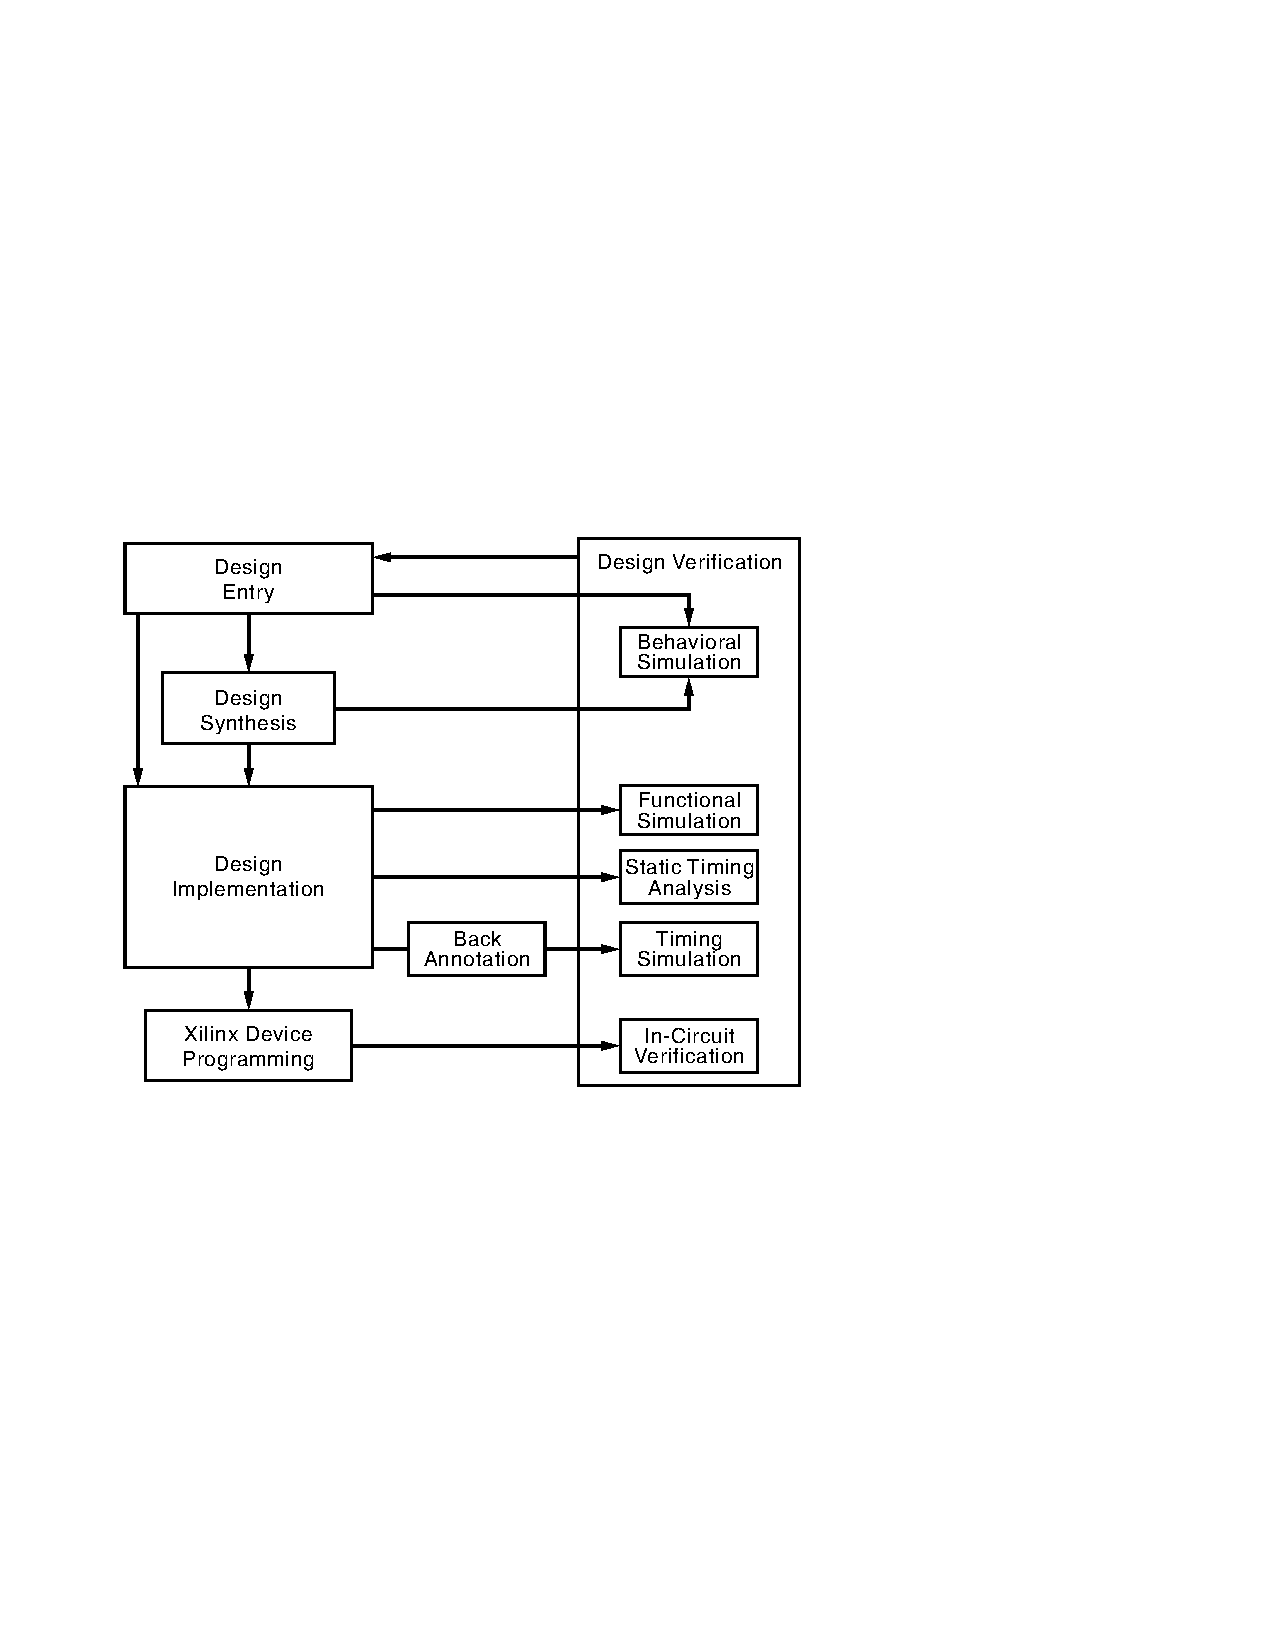
\includegraphics[width = 0.8\textwidth]{img/Round6_HardwareDiagram_overview}
	\caption{General hardware design flow \protect\cite{xilinx_manual}.}
	\label{fig:hardware_diagram}
\end{figure}

\vspace{11pt}
\textbf{The algorithms are re-written in HDL to ensure quality in hardware}

To implement the algorithms developed in MATLAB to HDL, we first tried using a software that automatically converts MATLAB code to Verilog. However, preliminary tests on the MATLAB generated Verilog showed that the code was of poor quality and difficult to  test and verify. Hence, to ensure a streamlined and power optimized chip, the algorithms were manually implemented in Verilog and fine-tuned. Figure \ref{fig:hardware_design_flow} shows Neurodetect’s version of the hardware design flow. The synthesis tool used in our design is ModelSim, an industry standard.

\begin{figure}[!ht]
	\centering
	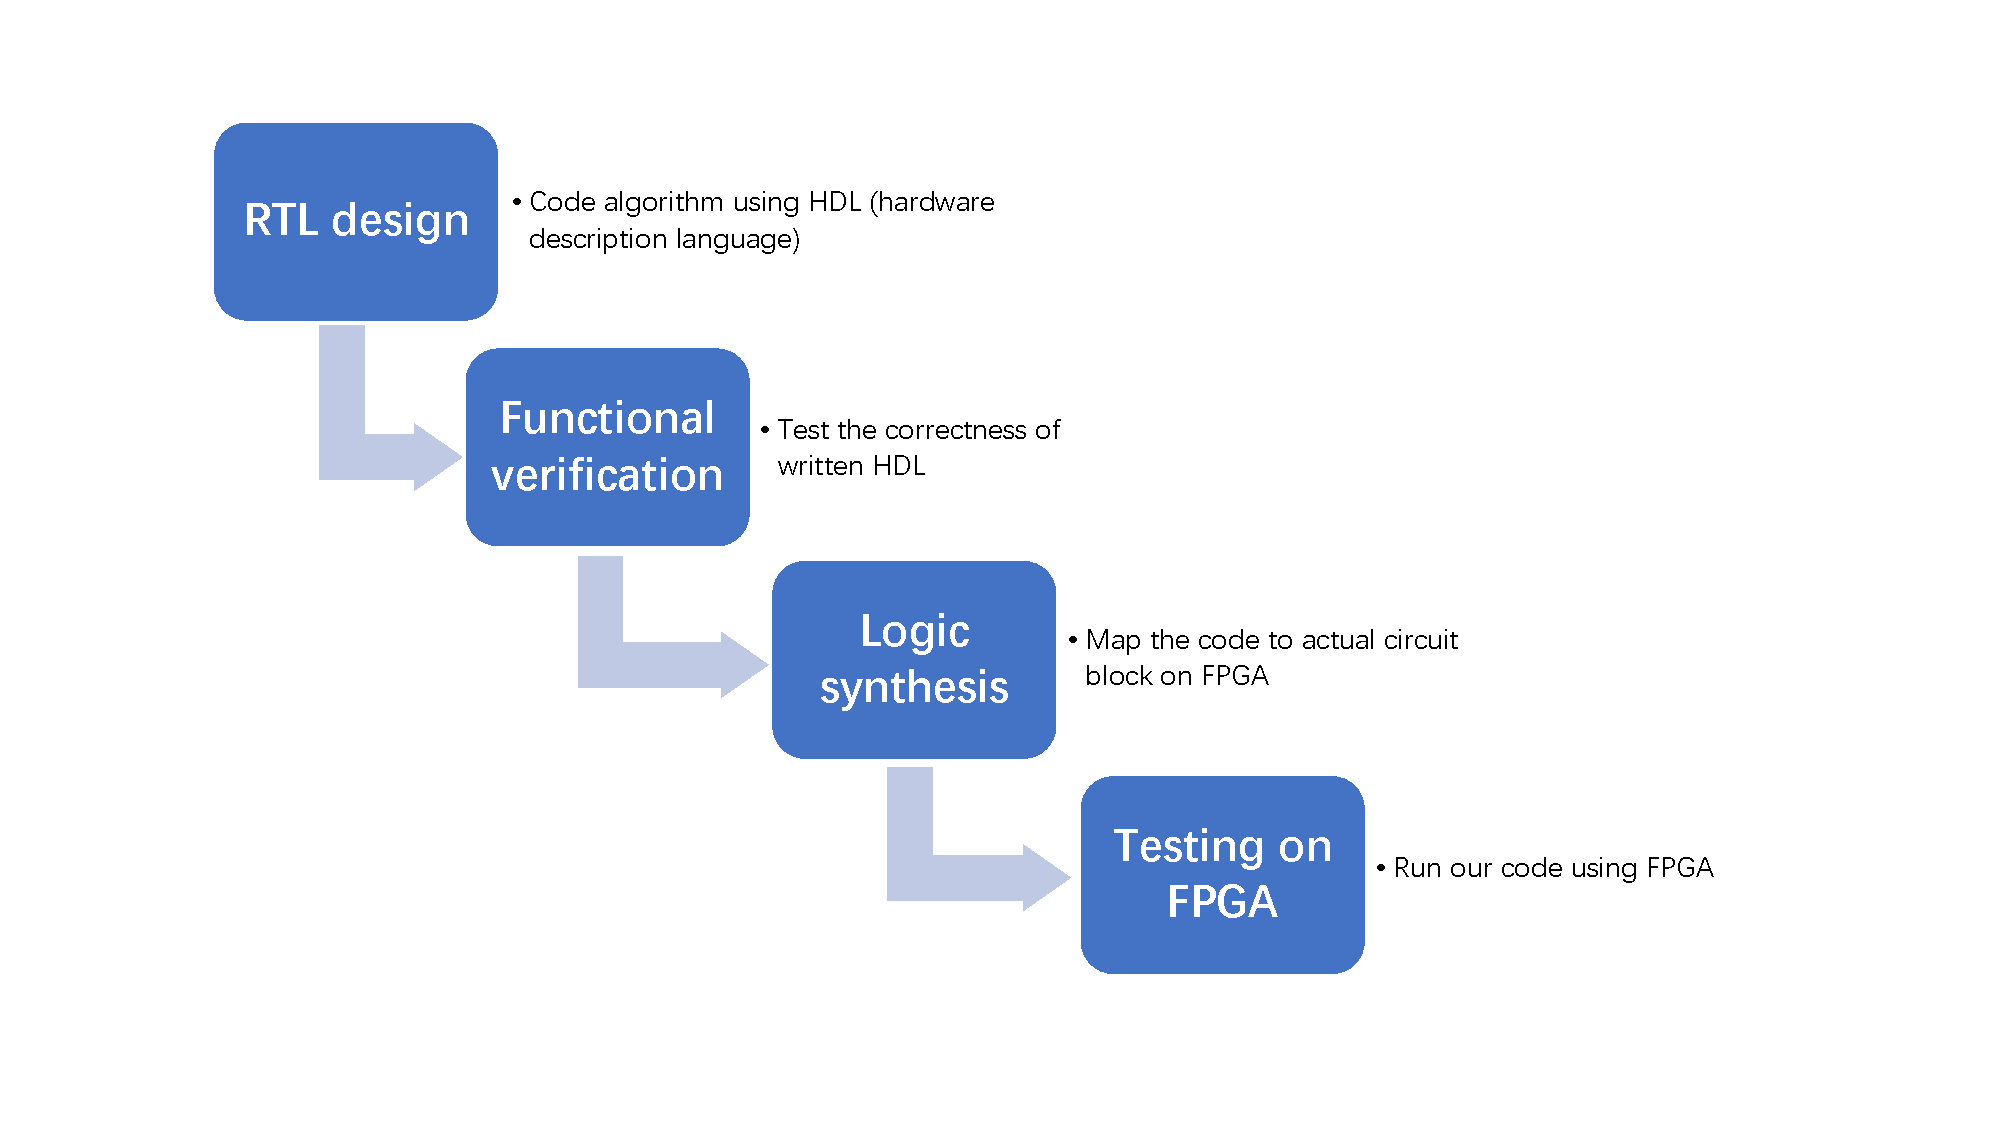
\includegraphics[width = \textwidth]{img/Round6_HardwareDiagram_design_flow}
	\caption{Substeps for implementing the detection algorithm on the FPGA.}
	\label{fig:hardware_design_flow}
\end{figure}

\newpage
\vspace{11pt}
\textbf{Designing at the RTL level allows for power optimization early in the design}

Registers are fundamental storage units in digital design. RTL focuses on how data flows between two registers and allows for significant power reductions very early in the design \cite{najm1995}. RTL abstraction is used in Verilog to create a high level representation of circuits that describes how data is processed and stored. Figure \ref{fig:linelength_rtl} illustrates the RTL design of the line length computation. The assortment of logical units shows of the datapath from input data to an output feature calculation that will then be used as part of the seizure detection. The accumulator and shift registers are common to all feature computations and make it so that we calculate the feature in a 1 second sliding window updated every 0.2 seconds. 

Initial simulation in a 32nm ASIC design demonstrated that our power consumption is about 2.4 nW per channel. ASIC refers to an application specific integrated circuit, which would be designed based on the FPGA implementation in order to produce the final chip. This number neglects to account for leakage which at these sizes would dominate our overall power.

\begin{figure}[!h]
	\centering
	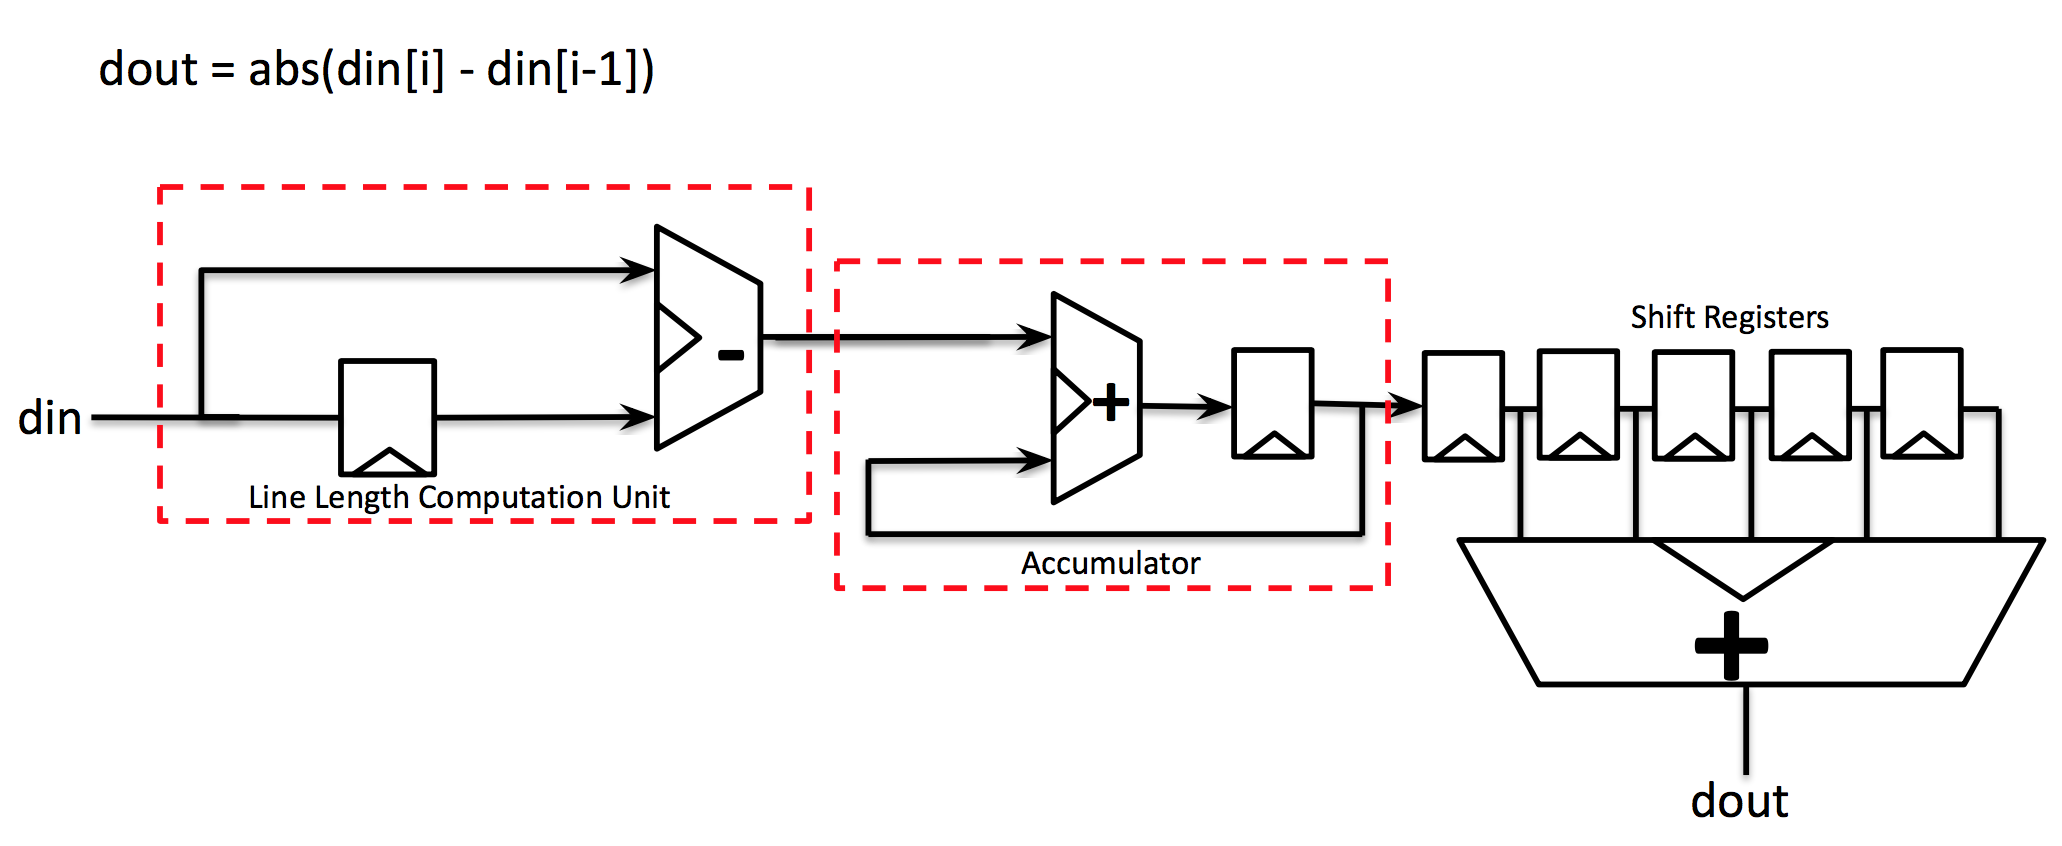
\includegraphics[width = 0.8\textwidth]{img/LL_RTL.png}
	\caption{Line length calculation RTL Flow} 
	\label{fig:linelength_rtl}
\end{figure}

\vspace{11pt}
\textbf{Design verification of the FPGA is a multistep process}
 
After generating the Verilog code, the preliminary design can be synthesized and then simulated. During synthesis, the code is mapped to millions of logical gates which allows the designer to perform gate-level simulation to test the design. Typical functional simulation is used to check if the circuit block behaves as intended and is done in several steps. First, a unit test is performed to ensure lower level components are functionally correct. For our seizure detection design, the lower level components consist of modules to calculate the line length, nonlinear energy, full-spectrum power and power in the theta, alpha and beta bands, as well as filters and a baseline computation module.The individual sub-component is implemented on the FPGA and tested against the simulated output from MATLAB to see if there is any significant difference between them.

Once each of the lower level components is individually verified, they are assembled to form the complete design and an overall test is performed. The overall test involves checking for problems in the functionality of the whole system and if any problems are found, the debug-redesign cycle is repeated until the system is bug-free. The datapath for our seizure detection instantiates each of the modules needed to compute the features from the iEEG data. The output of each computing module is fed to a controller which analyzes the results of each of the individual features calculated for multiple channels. By multiplying pre-calculated weights to the features, we are able to simulate results similar to those achieved by the software implementation of the algorithm. 

\vspace{11pt}
\textbf{Digital circuit timing analysis is paramount in ensuring fast yet reliable hardware }
 
Since Neurodetect's seizure detection chip must be both high speed and have low power consumption, timing analysis is critical to ensure that the chip is able to operate with low detection latency. In digital circuit design, digital circuits are separated into two categories: combinational logic and sequential logic. Combinational logic refers to circuits whose output is only dependent its current input while sequential logic refers to circuits whose output depends both on its current input and past inputs. To ensure that Neurodetect's chip works correctly, static timing analysis is performed after combining these two types of logic blocks to check that the input to different logic blocks arrive at the correct time.

\vspace{11pt}
\textsc{Conclusion}
\vspace{11pt}

Neurodetect is a complete seizure detection algorithm designed in both hardware and software. Initial testing on a limited dataset demonstrated a detection accuracy of 85\% with 0.7 false alarms per hour.

Neurodetect is helping to pave the way for future relatively simple seizure detection chips that can have a large impact on the lives of epilepsy patients. When the seizure detection module is combined with neural recording to obtain iEEG signals and stimulation or drug release to treat seizures, it provides a closed-loop solution to epilepsy.

Future directions for this project include deeper analysis on how to calculate the weights for the weighted sum. Specialized machine learning algorithms like Logistic Regression or Support Vector Machines might be better suited for classifying seizures. For hardware design, implementing the algorithm in an application-specific integrated circuit (ASIC) will result in lower power consumption.

%%%%%%%%%%%%%%%%%%%%%% BIBLIOGRAPHY %%%%%%%%%%%%%%%%%%%%%%%%%%%%%%

\clearpage
\bibliographystyle{apacite}
\bibliography{mybib.bib}

%%%%%%%%%%%%%%%%%%%%%% END DOCUMENT %%%%%%%%%%%%%%%%%%%%%%%%%%%%%%
\end{document}
